\documentclass{sigcomm-alternate}
\pdfpagewidth=8.5in
\pdfpageheight=11in

% added by Vaibhav
%----------------------------------------------------------------------
\usepackage{cite}
\usepackage[utf8]{inputenc}
\usepackage[table]{xcolor}
\usepackage[T1]{fontenc}
\usepackage[nolist]{acronym}
\usepackage{url}
\usepackage{todonotes}
\usepackage{booktabs}
\usepackage{listings}
\usepackage[font=footnotesize,caption=false]{subfig}
\usepackage[multiple]{footmisc}
\usepackage{color,soul}
\usepackage{amsfonts}
\usepackage{epigraph}
\usepackage[colorlinks=true,allcolors=blue]{hyperref}

\definecolor{gray}{gray}{0.93}
%----------------------------------------------------------------------

\begin{acronym}
  \acro{SDN}{Software Defined Networks}
  \acro{NV}{Network Virtualization}
  \acro{NFV}{Network Function Virtualization}
  \acro{DPDK}{Data Plane Development Kit}
  \acro{DDoS}{Distributed Denial-of-Service Attack}
  \acro{NSG}{Network Systems Group}
\end{acronym}


\begin{document}

\title{Munich Internet Research Retreat 2016}

%\numberofauthors{1}
%\author{
%\begin{tabular*}{0.9\textwidth}%
%{@{\extracolsep{\fill}}ccc}
%Vaibhav Bajpai & Arthur W. Berger & Philip Eardley \\
%\affaddr{Jacobs University} & \affaddr{Akamai Technologies} & \affaddr{British Telecom R\&D} \\
%\affaddr{Bremen, DE} & \affaddr{Cambridge, US} & \affaddr{Ipswich, GB} \\
%\email{v.bajpai@jacobs-university.de} & \email{awberger@csail.mit.edu} & \email{philip.eardley@bt.com}
%\end{tabular*}\\
%\begin{tabular}{c}
%\end{tabular}\\
%\begin{tabular*}{0.6\textwidth}%
%{@{\extracolsep{\fill}}cc}
%Jörg Ott & Jürgen Schönwälder \\
%\affaddr{TU München} & \affaddr{Jacobs University} \\
%\affaddr{München, DE} & \affaddr{Bremen, DE} \\
%\email{ott@in.tum.de} & \email{j.schoenwaelder@jacobs-university.de}
%\end{tabular*}\\
%\begin{tabular}{c}
%\end{tabular}\\
%\begin{tabular}{c}
%{\normalsize This article is an editorial note submitted to CCR. It has NOT
%been peer reviewed.}\\
%{\normalsize The authors take full responsibility for this article's
%technical content. Comments can be posted through CCR Online.}
%\end{tabular}
%}

\maketitle

\begin{abstract}

This article summarises a 2 day long research retreat seminar on  held in
November 2016.  The entire set of presentations delivered during the seminar
is made publicly available at \cite{mir-materials}.

\end{abstract}

% referrred: http://www.acm.org/about/class/ccs98-html
%\category{C.2.3}{Computer-Communication Networks}{Network Operations}[Network
%monitoring]

% referred: http://www.acm.org/sigs/publications/sigguide-v2.2sp
%\terms{Measurement, Performance}

\keywords{Internet measurements, Quality of experience, Network management,
Traffic engineering}

% sections
%----------------------------------------------------------------------
%**************************************************************************
\section{Introduction}\label{sec:introduction}
%**************************************************************************

%------------------------ Motivation
%------------------------ Goals

The goal of the workshop was to provide a forum for researchers in the Munich
area working on networking research to exchange ideas and develop further
collaoborations on similar interests.

In this workshop, we invited presentations on topics such as: (a) \ac{SDN},
(b) \ac{NFV}, (c) \ac{ICN}, (d) \ac{IoT}, (e) Internet measurements and (f)
security research.  On the basis of accepted proposals, the workshop was
organized in four sessions describing: (a) invited presentations, (b) parallel
group work, and (c) posters. We had 10 invited presentations on covering the
aforementioned topics and 11 posters presenting upcoming research. We also
organized 6 breakout sessions to discuss open topics in an informal setting.
A synopses of these four sessions appear in the upcoming sections below.

%**************************************************************************
\section{Invited Presentations}\label{sec:invited-presentations}
%**************************************************************************

The invited presentations were intended as a basis for triggering discussions
and identifying areas for group work.

% ------------ Dirk Kutscher
\subsection{Edge Computing considered harmful}


% ------------ Alexander von Gemler
\subsection{Towards A Clean Slate -- Digital Sovereignty in the Post Snowden Era}


% ------------ Artur Hecker
\subsection{On software network management}


% ------------ Wolfgang Kellerer
\subsection{FlexNets: Quantifying Flexibility in Communication Networks}


% ------------ Brian Trammell
\subsection{An Accidental Internet Architecture}


% ------------ Vaibhav Bajpai
\subsection{Measuring IPv6 Performance}


% ------------ Minoo Ruohi
\subsection{Path tracing and validation of IPv4 and IPv6 siblings}


% ------------ Laurent Vanbever
\subsection{SWIFT: Predictive Fast Reroute upon Remote BGP Disruptions}


% ------------ Christian Prehofer
\subsection{Open Platforms for Cyber-physical systems}


% ------------ Holger Kinkelin
\subsection{Collaborative intrusion handling using the Blackboard-Pattern}



%**************************************************************************
\section{Parallel Group Work}\label{sec:parallel-group-work}
%**************************************************************************

The afternoon sessions were used to discuss certain topics in more depth in
smaller groups. This section summarizes the discussions of each group.

% ------------- Andreas Blenk (TUM LKN)
\subsection{SDN/NFV Measurements}

With the introduction of \ac{SDN}, \ac{NV}, and \ac{NFV}, the programmability
and flexibility of our networks is promised to increase. With these new
concepts, networking tasks will be pushed on commodity hardware where they are
programmed as software.  However, this introduces new uncertainties in the
provided performance of these next generation networks as, in particular,
commodity hardware and software are not designed network processing.
Accordingly, new sophisticated measurement procedures are needed to benchmark
hardware and software components when faced with network packet processing.
Besides, as virtualization introduces an abstraction layer, this might come
with a performance overhead that needs to be considered and quantified. For
this purpose, existing measurement tools, such as MoonGen~\cite{pemmerich:imc:2015}, could be used to evaluate the performance for high
data rate with accurate precision.  Furthermore, tools designed for measuring
non-virtualized and virtualized \ac{SDN} networks (such as \texttt{perfbench}) could
measure the overhead of virtualization components, such as network
hypervisors. Measurements should be conducted on software platforms as well as
real networking testbeds. Hence, testbeds need to be built that include
commodity servers, e.g., making use of accelerated network cards via
\ac{DPDK}, networking functions in software, e.g., functions running in docker
containers, orchestration tools for virtual environments, e.g., HyperFlex~\cite{ablenk:im:2015} and OpenStack, as well as hardware that can generate
realistic network traffic, e.g., Spirent Test Center.  Generally, the
performance evaluation of virtualized networks and SDN networks is an
important task for the design of future communication networks.

% ------------- Georg Carle
\subsection{SDN++: Applications Perspective}

The breakout session entitled SDN++ dealt with SDN from the perspective of how
to apply SDN, and how to introduce improvements to SDN (thereby creating
SDN++), for better meeting the identified requirements.  Participants of the
breakout session were Laurent Vanbever, Artur Hecker, Wolfgang Kellerer,
Edwin Cordeiro and Georg Carle, the latter also being the presenter of the
results.  The method of the working group was first to identify relevant
application areas of SDN, then assess to which extent known SDN approaches
have shortcomings (i.e., identifying the `SDN pain areas'), and subsequently
identifying promising approaches for improving SDN\@.  The application areas of
SDN were (1) establishing means for programmability of the network, which can
be used for improving certain network properties, (2) management of advanced
cellular networks, in particular 5G networks, for different capabilities such
as network slicing, and (3) providing means to add sophisticated control
functionality to corporate networks, such as adding flexible access control.
Identified weaknesses of existing SDN were the fact that existing SDN
southbound interfaces, in particular OpenFlow, operate on a low level of
abstraction, which makes programming of the network time-consuming and error
prone.  Identified areas of improvement and need for further work were
specifying suitable high-level interfaces and abstractions.  There further is
the need to develop tools that are capable of automatically translate
high-level specifications to low-level configuration. A complete tool chain is
required.  This includes measurement tools that are capable of monitoring
changes. Network programmability is beneficial for measurement tools.  It is
expected that SDN management tools will facilitate to deal with the
programmability of networks.  Furthermore, verification tools will allow to
detect and prevent attempts of wrongly programming the network.    These tools
will form a network operating system, with tools that operate on top of the
operating system functions.  Another need for improvement is the development
of a clear transition path from today's networks to future SDN-based networks.
This includes to identify which legacy functionalities from today's networks
we assume being able to depend on in SDN deployments.


% ------------- Lars Eggert
\subsection{QUIC}

QUIC~\cite{draft-ietf-quic-transport} is a new UDP-based reliable transport
protocol with built-in security. The protocol is optimized for HTTP/2~\cite{rfc7540} that is currently being standardized by the \ac{IETF}. QUIC was
originally proposed by Google and has already seen large-scale deployment for
Google services and in Google Chrome. Since September 2016 a new IETF working
group reviews the design of QUIC in order to publish a QUIC protocol
specification with \ac{IETF} consensus. The break out session discussed how
the \ac{IETF} should approach on how the information encrypted in the QUIC
packets might be made available to legitimate network management or firewall
functions. The session also went into retrospect on historical protocol
innovations (such as HIP~\cite{pnikander:comst:2010} and SCTP~\cite{rfc4960})
that failed to get widely deployed to understand whether one needs to be
Google (or a large CDN player) to be able to deploy a protocol on the Internet
today. It was mentioned how good ideas and engineering also needs the right
incentives to see deployment and how partial deployability with one large CDN
player already brings benefits. QUIC is witnessing rapid adoption also because
Google controls both endpoints (browser and servers). As such, two endpoints
that can agree on an exchange that does not require middleware updates makes
it easier to deploy an innovation in practice, but still only influential
organizations have that leverage. Dave Thaler in~\cite{draft-iab-protocol-transitions} lays out strategies to allow smooth
transitions of future protocol innovations. Cost and benefit tradeoffs of
simpler deployability and clean-state designs were discussed. The deployment
incentives need to be aligned to allow early adopters to see the investment
benefits. It was also mentioned how operator networks remain opaque to
designers of network protocols and for the need for additional large-scale
measurement initiatives that help bring visibility into how current network
operate in practice would be useful for protocol innovation.

%Brian pointed to TSV area slides.

% Friday notes from Mirja:
% - if deployment incentives are not aligned, it
% - measurement provided by quic. Are additional measurements needed? Only few
%   can do this large-scale measurements. How valuable are measurements of
%   smaller networks (non-google).


% ------------- Johannes Naab / Heiko Niedermayer
\subsection{DDoS Defence beyond Centralization}

The danger of \ac{DDoS} attacks makes web services buy services of a few large
companies, such as Akamai or Cloudflare. Usually, this comes with a loss of
control on the side of the web service over defensive measures, e.g., blocking
which connections. Furthermore, we believe that this centralization of the
Internet is threatening the freedom of the Internet as users cannot bypass the
use of services of certain companies anymore. They lose their authority to
select the ones they want. In order to overcome this problem, we propose to
make \ac{DDoS} protection a service of ISPs to web services and in further
steps between ISPs and IXPs. If a web service is in trouble. It can alarm its
ISP and it can influence connections blocked by the ISP on its behalf. Details
need further research.

% ------------- Alexander von Gernler
\subsection{Security}

The security breakout session covered civil liberties and privacy. Firstly,
the group set its focus and decided not to discuss the topics of trustworthy
hardware or civil liberties, but instead to concentrate on \ac{SDN} security
and problems of cloudification. Key results: 1) Customer networks are
converging:  Customers want less own hardware, and want to be more independent
and to lease remote services and equipment rather than owning it.  2)
Virtualization (which happens when you cloudify applications) amplifies known
problems in traditional fields like security, trust, verifiability or
visibility.  3) A special challenge is the cloudification of services that
already utilize virtualization in the traditional model, for example sandboxes
that analyze malware.  For a cloud case, one would end up with nested
virtualization, which in turn comes with even new problems concerning
performance and visibility of the virtualization to the malware being
inspected 4) Encryption of data still leads to the usability of cloud
scenarios being reduced to mostly SaaS, because homomorphic encryption is
still not there to solve these problems 5) Special problems with end-to-end
security, e.g., there is more end-to-end encryption happening, which is good.
As a downside however, it makes life harder for people inspecting traffic in
the middle If termination of encrypted connections is done in the cloud, there
will be an unencrypted last mile as new security issue arising from this
scenario.

% ------------- Aaron
\subsection{IoT and ICN}

The breakout session on Internet of Things (IoT) and Information Centric
Networking (ICN) covered the open problems and research directions for
applying ICN technique to IoT. The identified problems include: 1) Limitation
of existing protocols such as Constrained Application Protocol (CoAP) that
handles poorly the frequent leaving/joining events in the network. 2) The
stereotype of ``IoT gateway design'' has hindered novel design. 3) We still
have not yet come up with a suitable Internet architecture that integrates
IoT coherently.

The group discussed how to bring ICN schemes to IoT, and highlighted several
open questions: 1) Where does the network end nowadays? This question couples
with the ICN where nodes can contribute to the computation/content along
the path. 2) What functions on gateway functions we can remove? 3) How to do
naming ``translation'' without changing name/label? 4) Can we do packet
processing while it is passing through queue? 5) How to avoid looping in
the network functions? This is a key concern since we need to keep a
boundary for resource usage in the network. 6) How to maintain the state on
the constrained nodes?

Regarding potential research directions, the group deem the following items
important: 1) Design of end-to-end naming scheme, to facilitate IoT
application composition and bring down the overhead of porting applications
for the cloud to "gateways". 2) Semantics for individual sensor and
equivalence group. 3) Trade accuracy with replication. 4) A new computation
abstract suitable for IoT. 5) Abstract of distributed registry for network
function. 6) Rethink how we distribute computing and content.

%**************************************************************************
\section{Posters}\label{sec:posters}
%**************************************************************************

Participants were also encouraged to volunteer for a lightning talk to provide
a perspective into their recent measurement research work.

% -------- Renata
%\subsection{HostView}

%**************************************************************************
\section{Posters}\label{sec:posters}
%**************************************************************************

Participants were also encouraged to volunteer to bring a poster to provide a
perspective into their recent measurement research work.

\subsection{The cost of Security in the SDN control Plane}

In OpenFlow enabled Software Defined Networks (SDNs) network control is
carried out remotely via a control connection. In order to deploy OpenFlow in
production networks, security of the control connection is crucial. For
OpenFlow connections TLS encryption is recommended by the specification. In
this work, we analyze the TLS support in the OpenFlow eco-system. In
particular, we implemented a performance measurement tool for encrypted
OpenFlow connections, as there is non available.  Our first results show that
security comes at an extra cost and hence further work is needed to design
efficient mechanisms taking the security-delay trade-off into account.

Published: R. Durner, W. Kellerer, The cost of Security in the SDN control
Plane, ACM CoNEXT 2015 - Student Workshop, Heidelberg, Germany, Dezember 2015.


\subsection{THE BALTIKUM TESTBED - Selected activities in the Baltikum Testbed}

The poster showed a high-level overview to the recent activities in the
Baltikum Testbed. The testbed which is focussed on performance measurements of
x86-based packet processing systems provides an automated, documented, and
reproducible experiment workflow. The poster presented several activities,
comprising the load generator MoonGen, automated benchmarks of routers and
OpenFlow switches, and different performance studies, including an IPsec
gateway with NIC-offloading.

Ref: [1] P. Emmerich, S. Gallenmüller, D. Raumer, F. Wohlfart, and G. Carle.
MoonGen: A Scriptable High-Speed Packet Generator. In Internet
Measurement Conference 2015 (IMC’15), Tokyo,
Japan, October 2015.
[2] Sebastian Gallenmüller, Paul Emmerich, Florian Wohlfart, Daniel
Raumer, and Georg Carle. Comparison of Frameworks for High-Performance
Packet IO. In ACM/IEEE Symposium on
Architectures for Networking and Communications Systems (ANCS 2015),
Oakland, CA, USA, May 2015.
[3] Daniel Raumer, Sebastian Gallenmüller, Paul Emmerich, Lukas Märdian,
Florian Wohlfart, and Georg Carle. Efficient serving of VPN endpoints on
COTS server hardware. In IEEE 5th
International Conference on Cloud Networking (CloudNet’16), Pisa, Italy,
October 2016.
[4] Daniel Raumer, Sebastian Gallenmüller, Florian Wohlfart, Paul
Emmerich, Patrick Werneck, and Georg Carle. Revisiting benchmarking
methodology for interconnect devices. In Applied
Networking Research Workshop 2016 (ANRW ’16), Berlin, Germany, 2016.


\subsection{Boost Virtual Network Resource Allocation: Using Machine Learning for Optimization}

Rapidly and efficiently allocating virtual network resources, i.e., 
solving the online Virtual Network Embedding (VNE) problem is 
important in particular for future communication networks. We 
propose a system using an admission control to improve the performance 
for the online VNE problem. The admission control implements a Neural 
Network that classifies virtual network requests based on network 
representations, which are using graph and network resource features 
only. Via simulations, we demonstrate that the admission control, 
i.e., the Neural Network filters virtual network requests that are 
either infeasible or that need too long for being efficiently 
processed. Thus, our admission control reduces the overall system 
runtime, i.e., it improves the overall calculation efficiency for 
the online VNE problem.
Generally, we demonstrate the ability to learn from the history 
of VNE algorithms. We show that it is possible to learn the behavior 
of algorithms and how to integrate this knowledge when solving future 
problem instances.

Reference:
[1] A. Blenk, P. Kalmbach, P. van der Smagt, W. Kellerer, Boost Online 
Virtual Network Embedding: Using Neural Networks for Admission Control,  
12th International Conference on Network and Service Management (CNSM),
 Montreal, Quebec, Canada, Oktober 2016.
%**************************************************************************
\section{Conclusions and Next Steps}\label{sec:conclusion}
%**************************************************************************

%!TEX root = ../index.tex

%**************************************************************************
\subsection*{Acknowledgements}\label{sec:acknowledgement}
%**************************************************************************

\begin{figure}[t!]
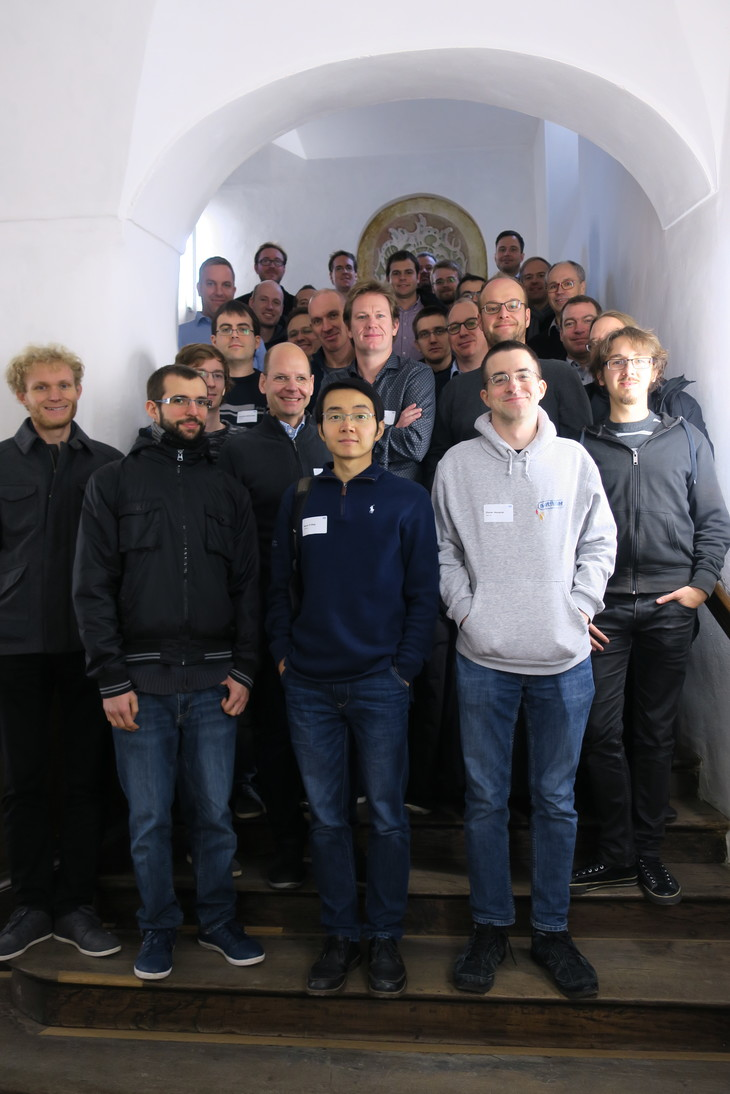
\includegraphics[width=\columnwidth]{figures/group-photo-scaled}
\end{figure}


This seminar was located at the TUM Science and Study Center in Raitenhaslach,
Germany, supported by NetApp, Huawei, and TUM\@.  The organizers would like to
thank the participants (alphabetically ordered by first name) for their
contributions---%
Aaron Yi Ding (TUM CM),
Alberto Martínez Alba (TUM LKN),
Alexander von Gernler (genua GmbH),
Andreas Blenk (TUM LKN),
Arsany Basta (TUM LKN),
Artur Hecker (Huawei),
Brian Trammell (ETH Zürich),
Christian Prehofer (fortiss, TUM),
Claas Lorenz (genua GmbH),
Daniel Raumer (TUM NET),
Dirk Kutscher (Huawei),
Edwin Cordeiro (TUM NET),
Florian Westphal (Red Hat),
Georg Carle (TUM NET),
Hagen Paul Pfeifer (Rohde \& Schwarz),
Heiko Niedermayer (TUM NET),
Holger Kinkelin (TUM NET),
Johannes Naab (TUM NET),
Jörg Ott (TUM CM),
Lars Eggert (NetApp),
Laurent Vanbever (ETH Zürich),
Marco Hoffmann (Nokia Bell Labs),
Markus Klügel (TUM LKN),
Matthias Wachs (TUM NET),
Minoo Rouhi (TUM NET),
Mirja Kühlewind (ETH Zurich),
Nemanja Djeric (TUM LKN),
Paul Emmerich (TUM NET),
Pavel Laskov (Huawei),
Peter Babarczi (TUM NET),
Raphael Durner (TUM LKN),
Rastin Pries (Nokia Bell Labs),
Rolf Winter (University of Applied Sciences Augsburg),
Sebastian Gallenmüller (TUM NET),
Vaibhav Bajpai (Jacobs University Bremen),
Wolfgang Kellerer (TUM LKN).

%----------------------------------------------------------------------

% bibliography
%----------------------------------------------------------------------
\bibliographystyle{abbrv}
\bibliography{index}
%----------------------------------------------------------------------

\end{document}
